%----------------------------------------------------------------------------------------
%	PACKAGES AND DOCUMENT CONFIGURATIONS
%----------------------------------------------------------------------------------------

\documentclass{article}

\usepackage[version=3]{mhchem} % Package for chemical equation typesetting
\usepackage{siunitx} % Provides the \SI{}{} and \si{} command for typesetting SI units
\usepackage{graphicx} % Required for the inclusion of images
\usepackage{natbib} % Required to change bibliography style to APA
\usepackage{amsmath} % Required for some math elements 
\usepackage{enumitem}% For lists
\usepackage{mathptmx}% For textbf
\usepackage{float} %for correct image placement
\usepackage{textcomp} % for texttildelow
\usepackage[T1]{fontenc} % allows use of less than <


\setlength\parindent{0pt} % Removes all indentation from paragraphs

\renewcommand{\labelenumi}{\alph{enumi}.} % Make numbering in the enumerate environment by letter rather than number (e.g. section 6)

%\usepackage{times} % Uncomment to use the Times New Roman font

%----------------------------------------------------------------------------------------
%	DOCUMENT INFORMATION
%----------------------------------------------------------------------------------------

\title{M152A - Lab 2 \\ Floating Point Conversion} % Title

\author{Markus \textsc{Notti} - 904269231 \\ Kyle \textsc{Baker}  - 604273748 \\ Niels \textsc{Pineda} - 604272353} % Author name


\date{\today} % Date for the report

\begin{document}

\maketitle % Insert the title, author and date

%----------------------------------------------------------------------------------------
%	SECTION 1
%----------------------------------------------------------------------------------------

\section*{Introduction}

In this lab, we implemented a basic floating point converter using Xilinx ISE software.  This converter takes a 12 bit signed integer and converts it to an 8 bit signed floating point number using rounding methods to keep the numbers as close to their true value as possible, as it is not possible to fully represent the full range of ints represented in a 12 bit signed integer. \\

Though the specific and immediate goal of this lab is to construct such a floating point converter, the overarching goal is to create a combinational circuit which performs the compression operation which maps a large signal to a smaller one.  This is essentially what is being done by creating the converter.

This lab was only implemented as a simulation, and in order to test it, we designed test bench files for the entire floating point converter as well as for each of the individual modules that we implemented.

Below I have included an image with the basic inputs and outputs of our floating point converter:

\begin{figure}[H]
\begin{center}
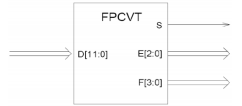
\includegraphics[width=0.8\textwidth]{fpcvtModulePic.png} 
\caption{fpcvt Module Basic Overview}
\end{center}
\end{figure}

As illustrated by the diagram above, the floating point converter module, called \textit{fpcvt} takes as input a 12 bit signal \textit{D} and outputs 3 separate signals, each a different component of the 8 bit floating point number that the module generates.  The first of the inputs \textit{S} is the sign bit. This bit is set to 0 when the number is positive and is set to 1 when the number is negative.  The second output generated is \textit{E}, a 3 bit signal representing the exponent component of the floating point number.  The third and final output generated is \textit{F}, a 4 bit signal representing the significand of the floating point number.  The resulting floating point number is therefore a combination of these three outputs and takes the following 8 bit form:

\begin{figure}[H]
\begin{center}
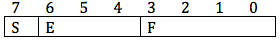
\includegraphics[width=0.8\textwidth]{floatingPointRep.png} 
\caption{fpcvt Module Basic Overview}
\end{center}
\end{figure}

The exponent and the significand work together to represent the magnitude of the number.  The significand represents the 4 most significant bits, while the exponent's purpose is to store the power to which 2 should be placed before multiplied with the significand to obtain the final magnitude of the final floating point number.  For further explanation, the resulting floating point number generated is obtained by the following formula where \textit{V} represents the final value of the generated floating point number: 

\begin{center}
\[ V  =  (-1)^S \times F \times 2^E \]
\end{center}

Some examples of this 8 bit floating point representation can be seen in the table below:

\begin{center}
\begin{tabular}{ c c c }

\textbf{Floating Point Representations}
 \textbf{Floating Point} & \textbf{Representation Formula} & \textbf{Value} \\ 
\big[0 000 0000\big] & 0 x 20 & 0\\  
\big[1 010 1010\big]  & -10 x 22 & -40 \\
\big[0 011 0111\big] & 7 x 23 & 56\\
\big[0 010 1110\big] & 14 x 22 & 56\\

\end{tabular}
\end{center}

In order to correctly implement this floating point converter, there are some special cases that must be considered.  The first of which is rounding.  This will occur quite often and must be considered.  Since the converter compresses the data from 12 bits to 8 bits, there are many numbers that cannot be represented by the final 8 bit number.  Therefore, the module must be able to handle cases where such numbers are compressed, and it does so by rounding.  In the process of conversion, the 4 most significant bits are taken and placed into the significand.  The 5th most significant bit is then taken and used to consider rounding.  If this 5th bit is 1, the significand is rounded up.  If the 5th bit is a 0, the remaining bits will be truncated, thus rounding the resultant number down.  Some examples of how the module implements rounding are included in the table below:

\begin{center}
\begin{tabular}{ c c c }

\textbf{Rounding Examples}
 \textbf{Linear Encoding} & \textbf{Floating Point Encoding} & \textbf{Rounding } \\ 
000000101100 & \big[0 010 1011\big] & Down \\
000000101101 & \big[0 010 1011\big] & Down \\ 
000000101110 & \big[0 010 1100\big] & Up \\
000000101111 & \big[0 010 1100\big] & Up \\

\end{tabular}
\end{center}

Another, but a more specific, outlying case that must be dealt with is when the significand is rounded up, but the significand consists of 4 1's. When this occurs, the exponent is incremented by 1 and the significand is first right shifted by 1 and then incremented by 1.  This successfully completes the rounding.  There is one even more specific case of rounding occurring when the exponent is incremented due to rounding, but it already contains all 1's. The converter module in this situation does not increment or shift either the exponent or the significand, because doing so would result in a garbage number.  This last example occurs when the input to the converter is too large of a number to be represented in 8 bit floating point form. Therefore, it logically follows that the final floating point number generated should have a magnitude with all 1's as this is the greatest possible magnitude that it is able to hold.

 
%----------------------------------------------------------------------------------------
%	SECTION 2
%----------------------------------------------------------------------------------------

\section*{Design Description}

% TODO: Make circuit diagram
% TODO: Make sure the figures referenced are correct

When designing the lab, we created a module for each section in figure 3. We named these modules convertToSignMag, countLeadZeros, extractLeadBits, and rounding to correspond to each of the sections in the figure. We then created a main module called fpcvt to tie all the other modules together. The implementation of the modules is described in the sections below.

\subsection*{fpcvt}
We then created a main module we named fpcvt which took in as input D, a bus of 12 wires and outputted a sign bit S, the exponent bus E, and the floating point bus F. The functionality of fpcvt essentially just followed the flow of figure 3. We decided to follow this flow because it seemed the most logical and modular approach to solving the problem. The input D was passed into convertToSignMag, which fed its output to both countLeadZeros and extractLeadBits. The output of extractLeadingBits (the significand and the fifth bit) and the output of countLeadingZeros (the exponent) were passed into the rounding module. We then assigned the output of the rounding function to E and F, the outputs of fpcvt.

\begin{figure}[H]
	\begin{center}
		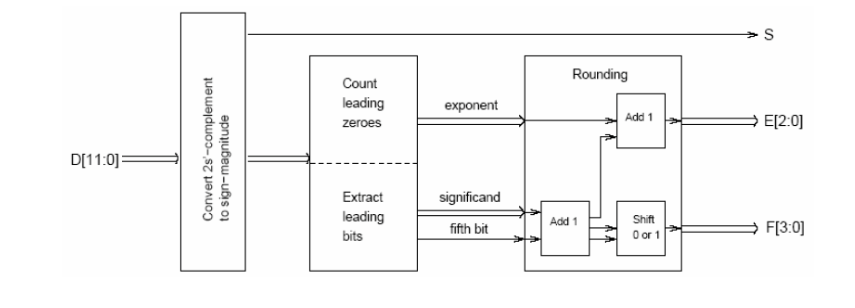
\includegraphics[width=1\textwidth]{overall_design_ideas.png} 
		\caption{fpcvt design diagram from lab.}
	\end{center}
\end{figure}

The circuit diagrams for each of the sections in the figure above will be depicted in the following sections.

\subsection*{convertToSignMag}
Our convertToSignMag module took in an 12 bit input named D2 and and has S2 and MAG as 1 and 11 bit outputs respectively. D2 represents the original 12 bit input into the fpcvt module, S2 represents the sign bit to be outputted in fpcvt, and MAG represents the unsigned magnitude of the 12 bit integer passed in. The first step in this module was creating a 12 bit reg called tempMAG which we assigned to have the same value as D2 in order to operate on D2. We then checked if D2 was equal to the bit stream 100000000000, which is the most negative number. We needed to check this because the next step is, if the number is negative, inverting the number by taking its complement and adding one. But since the integer can only represent numbers in the range -2048 to 2047, overflow will occur. In this case, we set our sign bit to 1 and our magnitude to 11111111111 and return from there. Otherwise, we checked if the sign bit was negative. If it was, we inverted tempMAG as previously mentioned. We then used a for loop to extract the 11 least significant bits in order to extract the magnitude and ignore the sign bit. In the end, we assigned the output MAG to be tempMAG and the sign bit output S2 to be D2[0] (the first bit of the input integer).

\begin{figure}[H]
	\begin{center}
		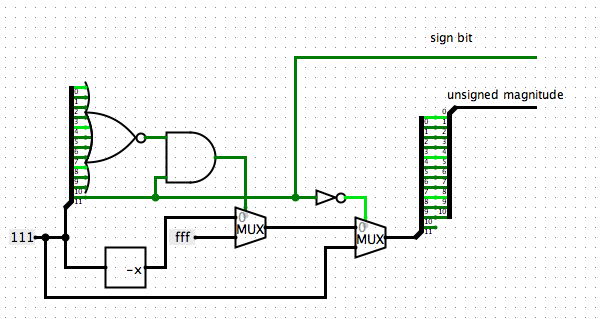
\includegraphics[width=1\textwidth]{convertToSignMag.png} 
		\caption{convertToSignMag circuit diagram}
	\end{center}
\end{figure}

In this circuit, the input is 12 bits (represented in hex on the diagram) and the output is one sign bit and one bus of 11 bits which is the unsigned magnitude. The 11 least significant bits are fed through a NAND gate to find out of they are all zeros. That signal is then fed to an AND gate along with the sign bit. The purpose of this is to find out if the input is the most negative integer, 100000000000. In this case, we have the output be 111111111111, or fff in hex on the diagram. Otherwise, we use a mux to choose between the inverted version of the integer and the regular version of the integer depending on whether the sign bit is 1 or 0. At the end, we extract all the bits but the sign bit to get the unsigned magnitude.

\subsection*{countLeadZeros}
The countLeadZeros module takes in MAG3 as an 11 bit input and specifies E3 as a 3 bit output. MAG3 represents the magnitude of the integer passed into the fpcvt module and E3 represents the exponent of the integer. The exponent E3 was calculated by counting the number of leading zeros, then setting E3 to the corresponding exponent value in the table below.

\begin{figure}[H]
	\begin{center}
		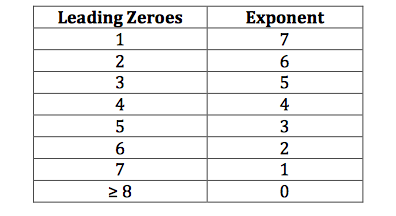
\includegraphics[width=.6\textwidth]{exponent_table.png} 
		\caption{Leading zeros to exponent conversion table taken from the lab.}
	\end{center}
\end{figure}

To count the number of leading zeros, we used a priority encoder. We utilized a switch statement to implement the priority encoder. We first checked the first leading bit. If that bit was 1, then there was 1 leading zero (including the sign bit). If it was zero, then we check the next bit. If that bit was 1, then there were 2 leading zeros, and so on. With this information, we assigned the proper exponent value to E3.

\begin{figure}[H]
	\begin{center}
		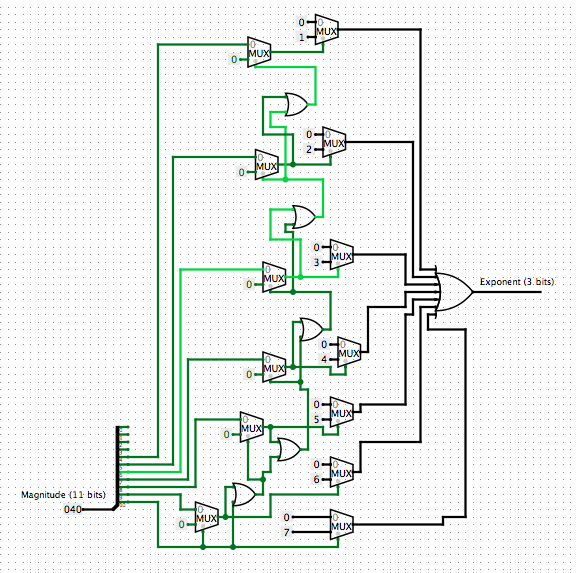
\includegraphics[width=1\textwidth]{countLeadingZerosCircuitD.png} 
		\caption{countLeadZeros circuit diagram}
	\end{center}
\end{figure}

The countLeadingZeros module in the circuit diagram above takes an 11 bit magnitude which is immediately split into its 11 bits.  These 11 bits then are sent into a cascade of muxes which essentially examine each bit one at a time, starting with the most significant.  As soon as a 1 bit is found, the cascade shuts down, and only the appropriate number, corresponding the appropriate amount of leading zeros, is chosen by a mux and finds its way to the 7 input OR gate, and then to the output as the 3 bit exponent.

\subsection*{extractLeadBits}
This module takes in MAG4 as a 11 bit input and specifies SIG4 as a 4 bit output and FB4 as a 1 bit output where MAG4 is the same as MAG3 in countLeadZeros. SIG4 represents the significand and FB4 represents the fifth bit. To calculate SIG4 and FB4, we first needed to left shift MAG4 by the number of leading zeros (up to 7 times). We then used another priority encoder (as described under countLeadZeros) to count the number of leading zeros and to decide how many times to left shift MAG4. We then assigned SIG4 to the four must significant bits of the shifted MAG4 and FB4 to be the fifth most significant bit of the shifted MAG4.

\begin{figure}[H]
	\begin{center}
		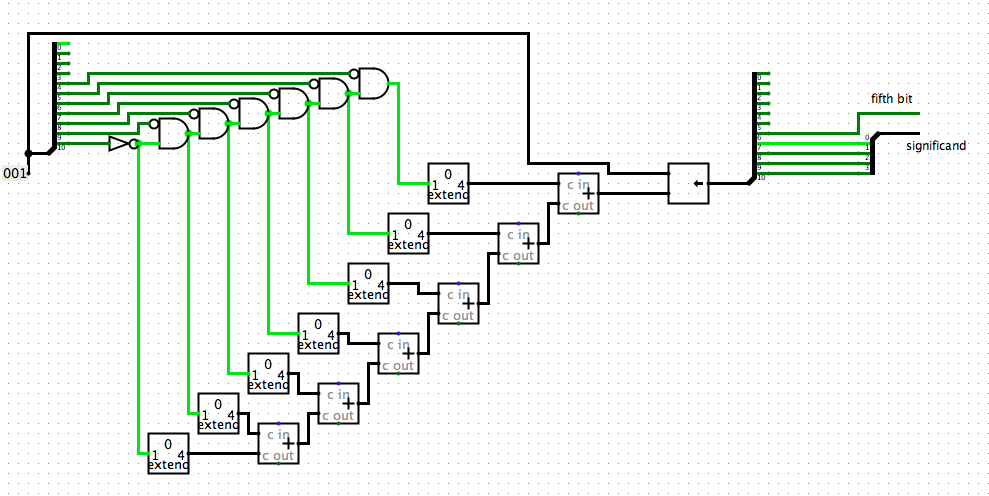
\includegraphics[width=1\textwidth]{extractLeadingBits.png} 
		\caption{extractLeadBits circuit diagram}
	\end{center}
\end{figure}

In the circuit diagram for extractLeadBits, we used a chain of ANDs with one input negated in order to count get a high signal on all the leading zeros and a low signal on all bits including and after the first 1 in the input. We only needed to count up to seven because seven is the max amount you can shift by. These signals are fed into a bit extender in order to make them 4 bits long to make them compatible with the adder in Logisim. All the signals are then added, thus giving a count of the number of leading zeros. After this, we feed the input and the count to a shifter and left the input shift by the count. From there, we extract the 4 most significant bits to get the significand and the fifth most significant bit to get the fifth bit.

\subsection*{rounding}
Our rounding module takes in E5 as a 3 bit input, SIG5 as a 4 bit input, and FB5 as a one bit input. E5 represents the exponent bus outputted by countLeadZeros and SIG5 and FB5 represent the significand bus and the fifth bit, both of which are outputted by extractLeadBits. The rounding module also specifies E6 as a 3 bit output and F6 as a 4 bit output. E6 and F6 represent the final exponent and significand values to be outputted by fpcvt. We began the module by checking if the significand was 1111 and the fifth bit was 1. This is important because when you add the two you'd get overflow, so we set a special overflow flag to be 1. In this case, we also checked to see if the exponent had the value 111 because when you add 1 to the exponent in this case you would overflow the exponent. If this case were true, we set a special flag we called "allOnes" to be true. If allOnes was true, we left the SIG5 and E5 unaltered because it was beyond what floating point could represent. If FB5 is zero, we also leave SIG5 and E5 unaltered because you just add by zero. If FB5 was one and overflow is zero, we simply added one to SIG5. If FB5 was one and the overflow bit was also one, then we shifted SIG5 right by one, added one to the exponent, and added one to the already shifted SIG5. We had to shift before we added to SIG5 because if we added first, overflow would happen and zero out SIG5. At the end, we assigned E6 and F6 to the manipulated E5 and SIG5 values.

\begin{figure}[H]
	\begin{center}
		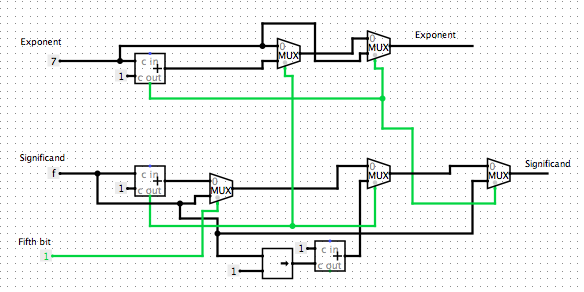
\includegraphics[width=1\textwidth]{RoundingCD.png} 
		\caption{rounding circuit diagram}
	\end{center}
\end{figure}

The rounding module in the circuit diagram above takes as input a 3 bit temporary exponent, a 4 bit temporary significand, and a 1 bit ``fifth bit''.  The exponent and significand are immediately incremented and sent into muxes each with their original un-incremented selves where the fifth bit input is chosen as the selector for the significand, telling the mux to use the incremented significand if 1.  The overflow of that addition is then used as the selector for the mux with the exponent and its incremented self as input.  If the significand's overflow is then also used as the selector for another mux which, if overflow is 1, sets its output equal to the original significand right shifted and incremented.  Another mux then handles the case of the exponent and significand both overflowing, resetting the outputs to all 1's. 

%----------------------------------------------------------------------------------------
%	SECTION 3
%----------------------------------------------------------------------------------------

\section*{Simulation}

The simulation portion of the lab involved several test bench files, one for each individual module, with the most thorough of the test cases falling under the overarching FPCVT.  By understanding what each module was intended to do, and thus knowing the expected output for each one, the testing simply consisted of: creating a test bench file via adding a ``testing fixture'' source, then writing example instances along with a delay in said file, and finally running through the iSIM Waveform while checking accuracy by hand. Our individual modules, which more or less acted as ``sub/helper-functions'' in order to implement the overall module of FPCVT, consisted of: convertToSignMag, countLeadZeros, extractLeadBits, and rounding.  While it may not have been the best idea, we made very simple and basic test cases for these smaller modules in order to allow us to continue to progress in a timely fashion, while still working at a timely rate.  \\ 

For convertToSignMag, the input was the input data in the form of two's complement.  The two instantiations we tested were the integer values of 1 and -1, or D2 = 12'b000000000001 and D2 = 12'b111111111111 respectively.  We felt as though these were good, simple test cases as they were several corner cases which also tested if both our negative and positive conversion was working correctly.  As expected, the outcomes were correctly stored in S and MAG: for 1 S=0 and MAG=00000000001 and for -1 S=1 and MAG=00000000001.     

\begin{figure}[H]
	\begin{center}
		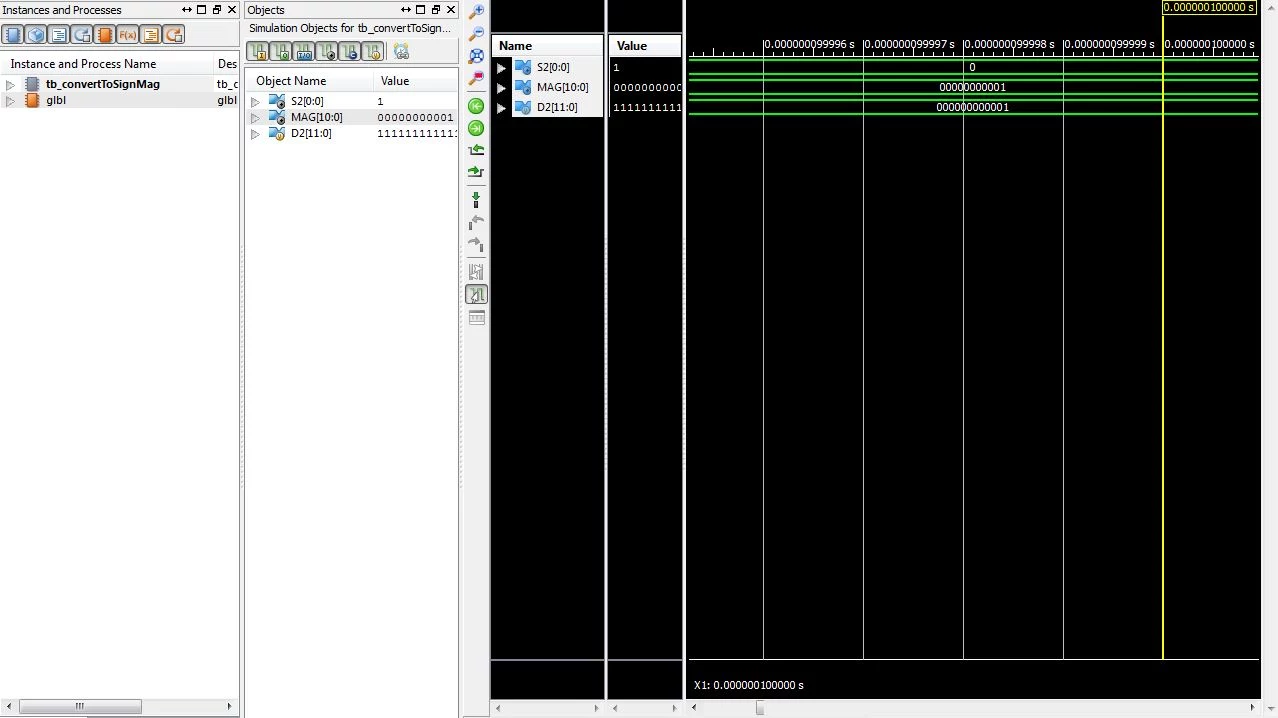
\includegraphics[width=1.2\textwidth]{sim1.png} 
		\caption{Example testbench simulation testing convertToSignMag module}
	\end{center}
\end{figure}

The following simulation for countLeadZeros was by far the trickiest for our group, as we initially had trouble understanding exactly what the output was to look like; consequently, this led to us believing our first attempt was correct which made our overall converter fail.  However, after clarifying the process for this module, we were able to produce the correct output, in which we checked many cases including: MAG3 = 11'b00000000000; MAG3 = 11'b00000000001; MAG3 = 11'b00000000010; MAG3 = 11'b00000000100; MAG3 = 11'b00000001000; MAG3 = 11'b00000010000; MAG3 = 11'b00000100000; MAG3 = 11'b10100100000; and MAG3 = 11'b11111111111.  Our initial approach led to undefined behavior, but after the fix, we were very thorough in testing this module.  All of these test cases simply represented every different number of leading zeros (from 0 to > 8) which would led to different exponents.

\begin{figure}[H]
	\begin{center}
		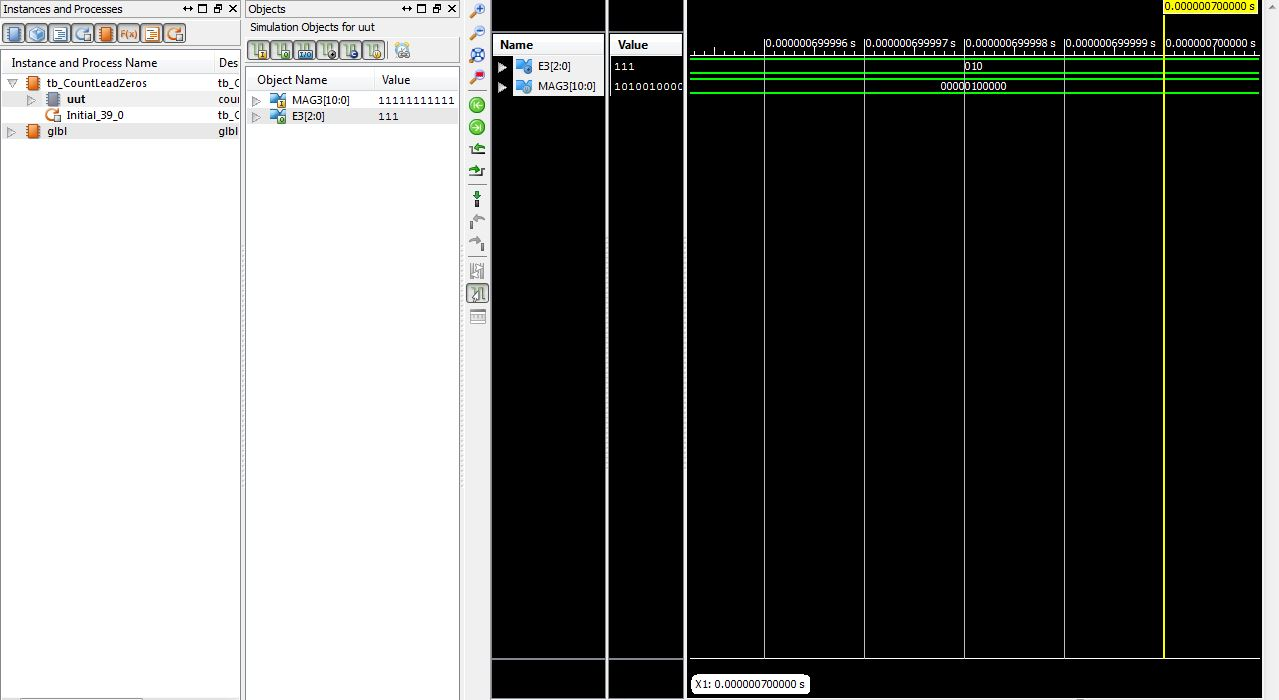
\includegraphics[width=1.2\textwidth]{sim2.png} 
		\caption{Example testbench simulation testing countLeadingZeros module}
	\end{center}
\end{figure}

Module extractLeadBits was relatively straightforward, and similarly, so were the test cases.  Because of the simplicity of the code itself, which merely consisted of a priority encoder, we only used two test cases, which were passing in the magnitude (MAG4) as MAG4 = 11'b01101000101 and MAG4 = 11'b00000101111.  These represented relatively simple cases that assured our priority encoder was working, and both of these resulted in the expected outcomes.


\begin{figure}[H]
	\begin{center}
		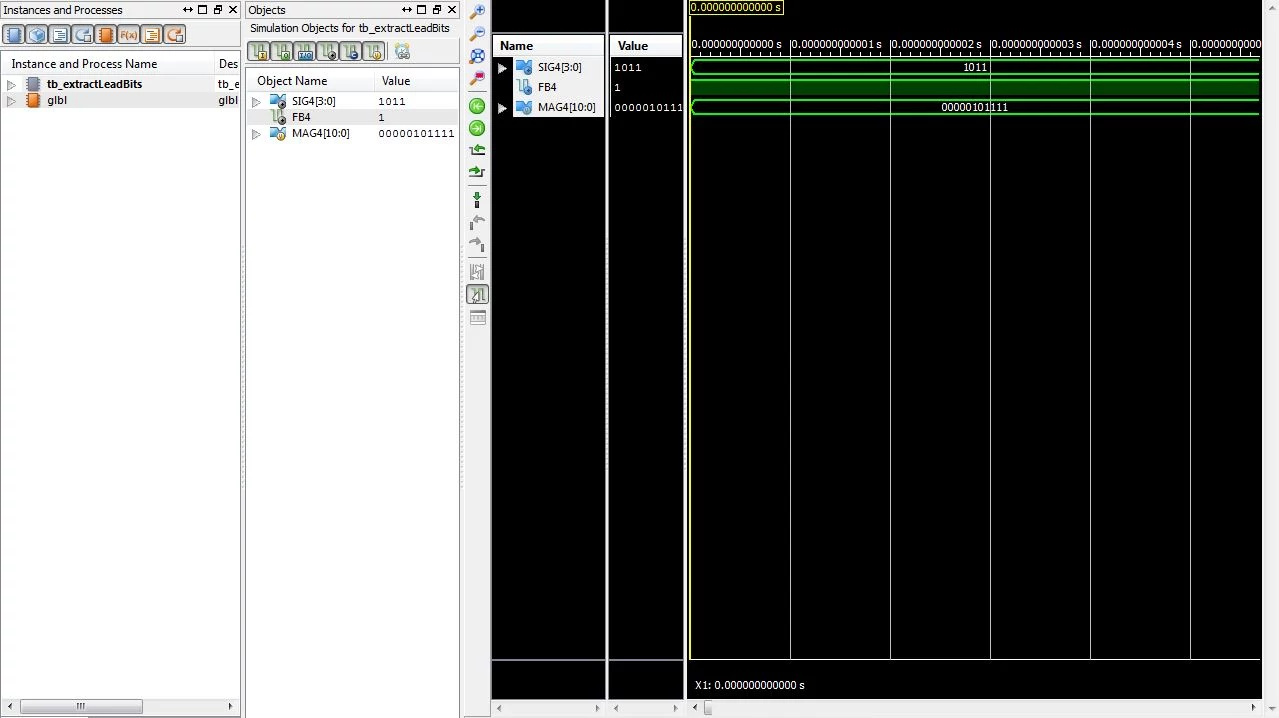
\includegraphics[width=1.2\textwidth]{extractLeadingBitsSim.png} 
		\caption{Example testbench simulation extractLeadBits module}
	\end{center}
\end{figure}


The final module (aside from the converter) was used for rounding of the floating point conversion.  We carefully tested the various corner cases (in this case, the various types of overflow) after testing a couple of very basic cases.  The cases we tested were based off of changing the exponent (E5), significand (Sig5) and fifth-bit (FB5); the cases included: [E5 = 3'b001; SIG5 = 4'b0001; FB5 = 0;] ; [E5 = 3'b001; SIG5 = 4'b0001; FB5 = 1;] ; [E5 = 3'b001; SIG5 = 4'b1111; FB5 = 1;] and [E5 = 3'b111; SIG5 = 4'b1111; FB5 = 1;].  The first two instantiations were very simple cases, simply assuring if the basic rounding was correct.  Once those were verified, we tested two major overflow conditions, one in which the exponent could had room to carry over, and the other where there was no room for adding to any input.  These covered the major corner cases, all of which eventually passed with some adjustments to the code to account for those particular cases. 

\begin{figure}[H]
	\begin{center}
		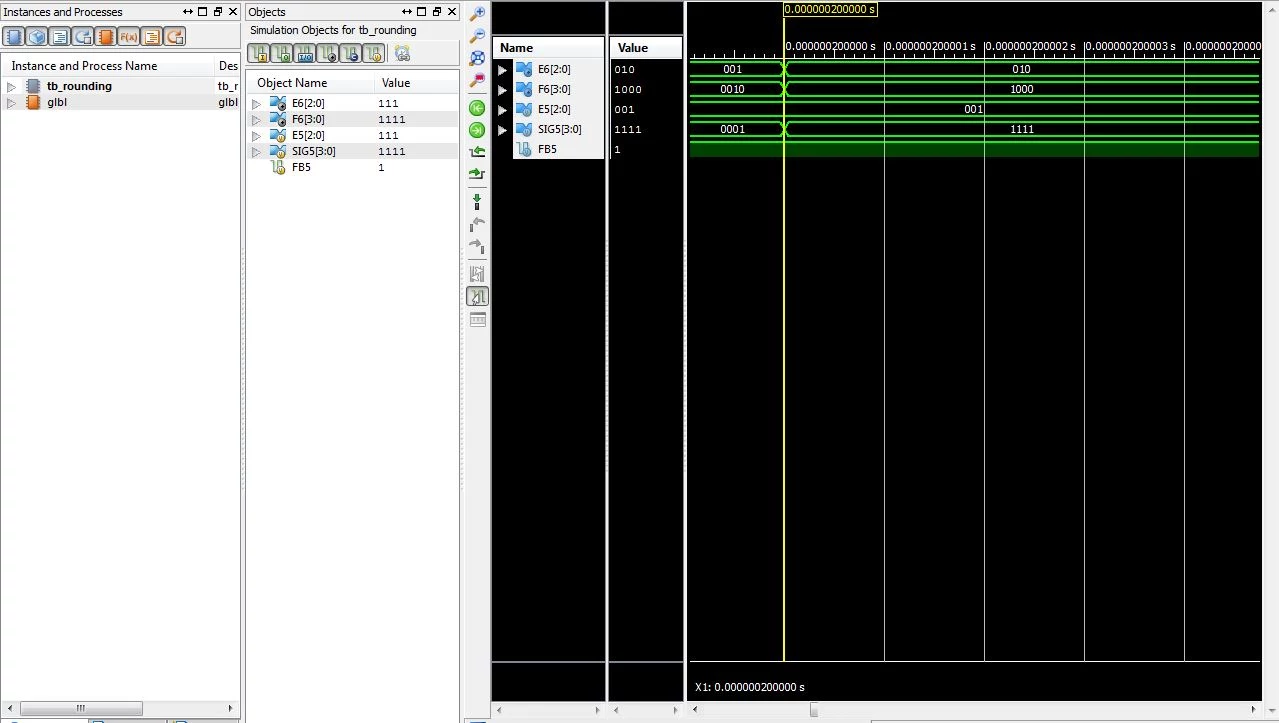
\includegraphics[width=1.2\textwidth]{sim5.png} 
		\caption{Example testbench simulation testing rounding module}
	\end{center}
\end{figure}

Lastly, and most importantly, we tested the entire converter, FPCVT.  The major trouble we had testing this came when we believed all of our sub-modules were working correctly, when in fact countLeadZeros was not outputting what it was supposed to.  After that adjustment, our test simulations were generally correct aside from a single corner case (which was the most negative number).  We had a variety of test cases including: D = 12'b 000000101100; D = 12'b 000000101101; D = 12'b 000000101110; D = 12'b 000000101111; D = 12'b 111111111111; D = 12'b 011111111111; D = 12'b 011111000000; D = 12'b 100000000000; D = 12'b 111001011010, where D was the input.  As indicated by the images below, these test cases checked for multiple conditions including: the base case of a generic number (000000101110), negative rounding (111001011010), negative one (111111111111), the most positive number (011111111111), and the edge case (which is the one we initially missed) of 100000000000. 

\begin{figure}[H]
	\begin{center}
		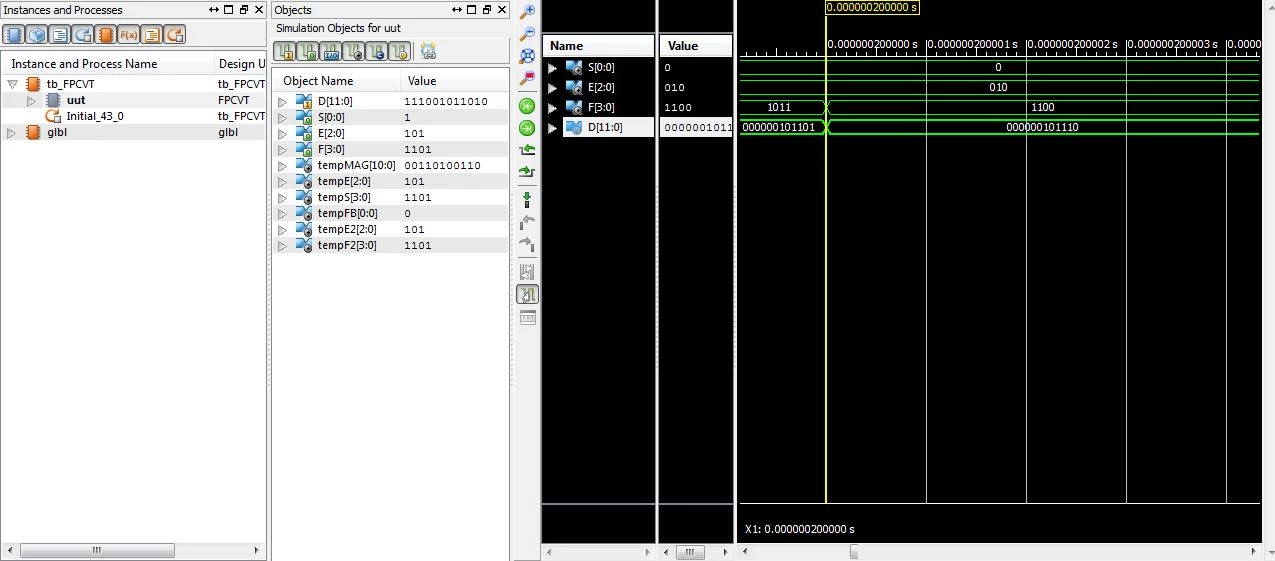
\includegraphics[width=1.2\textwidth]{sim3.png} 
		\caption{Example testbench simulation testing generic number on fpcvt module}
	\end{center}
\end{figure}

\begin{figure}[H]
	\begin{center}
		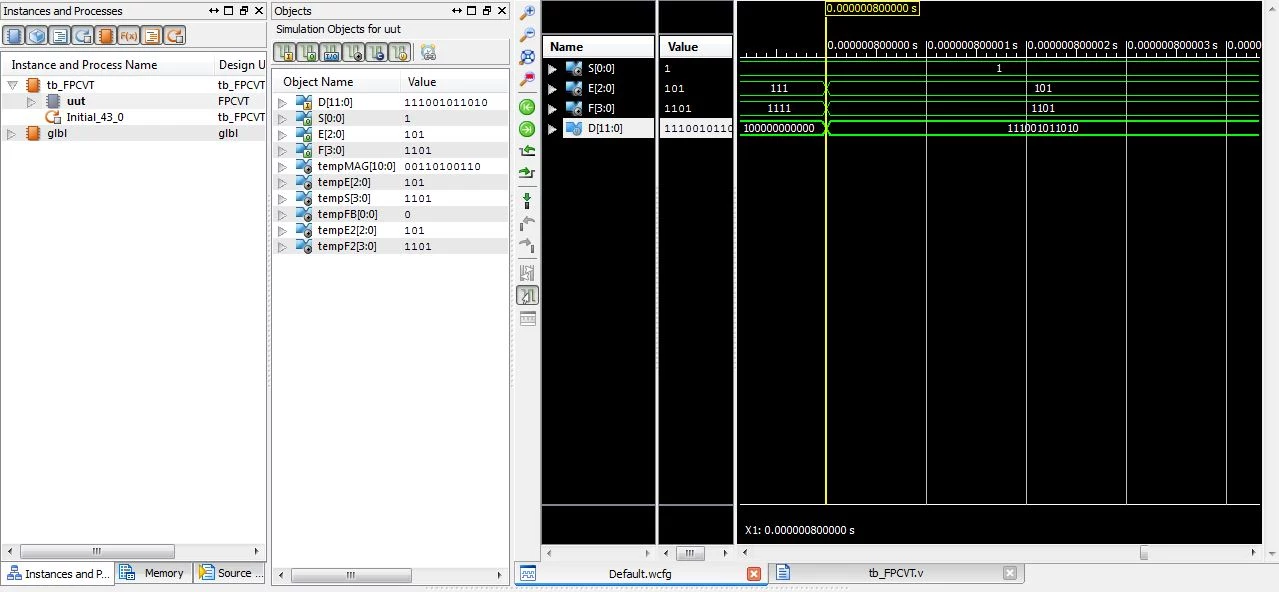
\includegraphics[width=1.2\textwidth]{sim4.png} 
		\caption{Example testbench simulation testing negative rounding on fpcvt module}
	\end{center}
\end{figure}

\begin{figure}[H]
	\begin{center}
		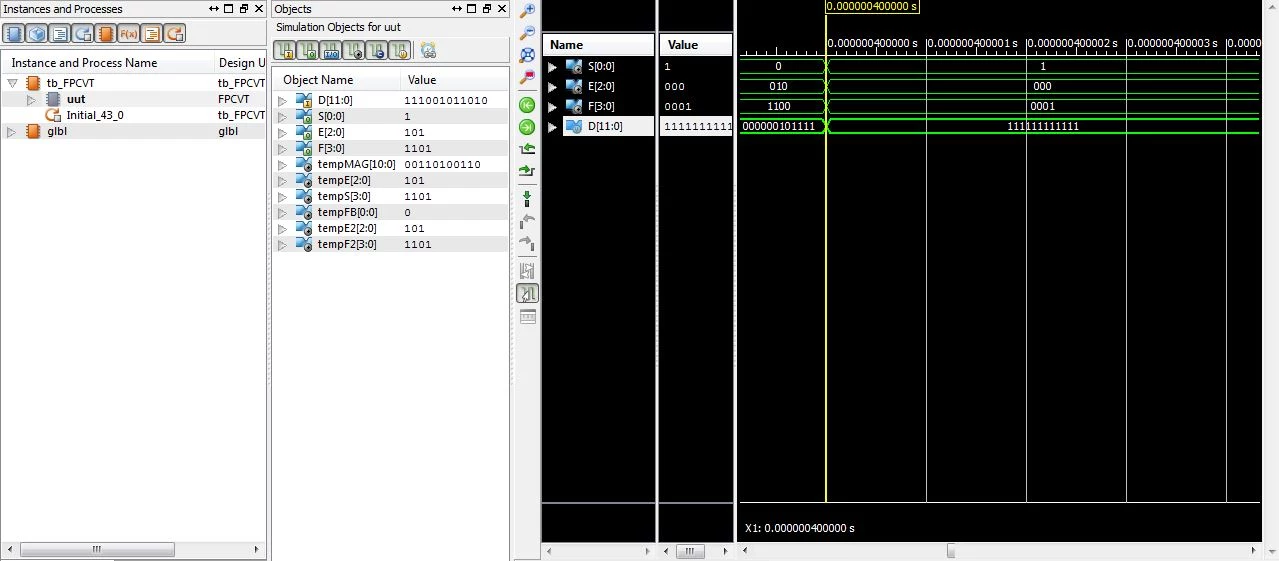
\includegraphics[width=1.2\textwidth]{sim7.png} 
		\caption{Example testbench simulation testing negative 1 on fpcvt module}
	\end{center}
\end{figure}

\begin{figure}[H]
	\begin{center}
		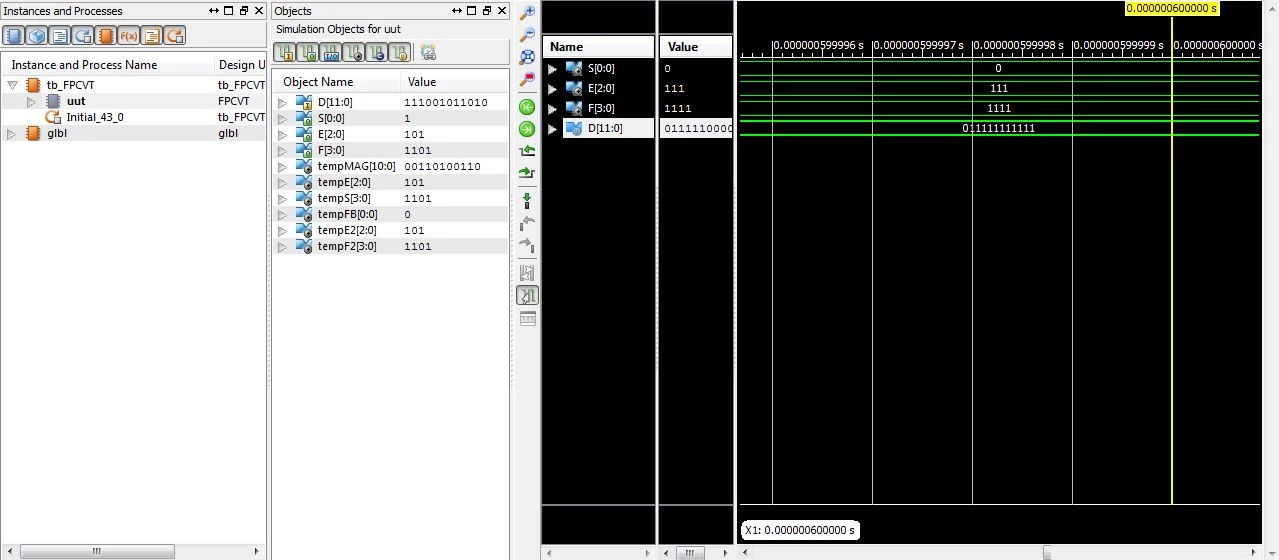
\includegraphics[width=1.2\textwidth]{mostPositiveSim.png} 
		\caption{Example testbench simulation testing most positive number on fpcvt module}
	\end{center}
\end{figure}

\begin{figure}[H]
	\begin{center}
		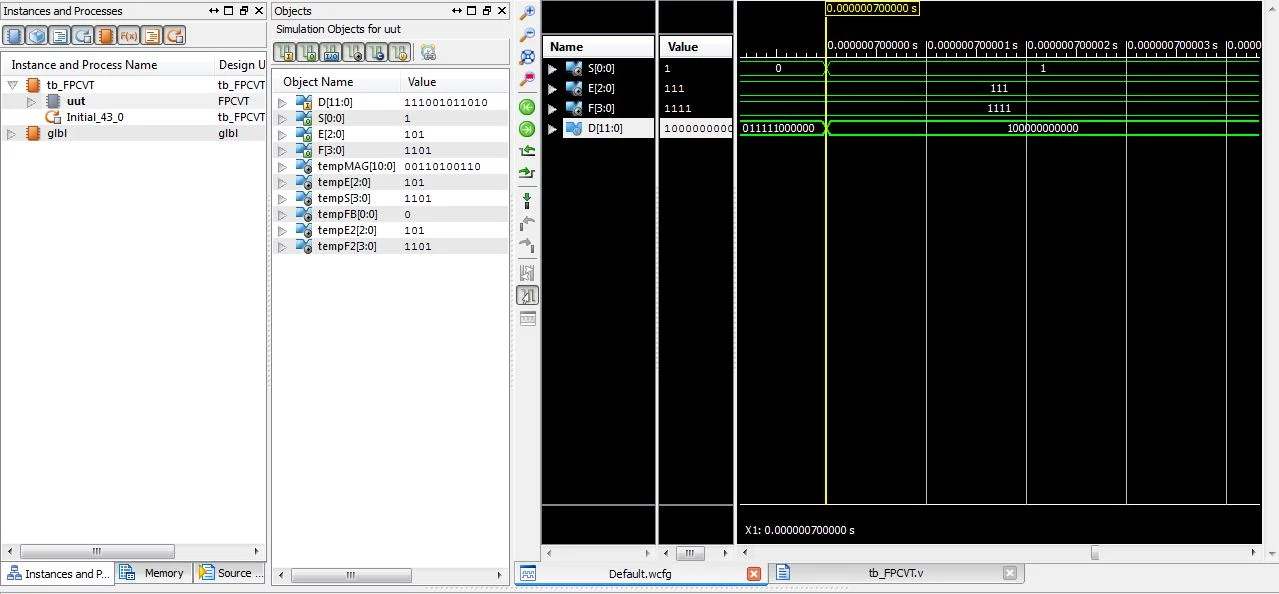
\includegraphics[width=1.2\textwidth]{sim6.png} 
		\caption{Example testbench simulation testing edge case on fpcvt module}
	\end{center}
\end{figure}

\section*{Conclusion}

Overall, the implementation of the converter went relatively smoothly, especially with the help of the lab manual.  By breaking down the the overall design and module of FPCVT into several modules, in our case: convertToSignMag, countLeadZeros, extractLeadBits, rounding, then using all of them in the, the process was made much clearer and easier.  Initially, we fed in the data in two's complement representation into the convertToSignMag.  That module's output was used as the input to countLeadZeros and extractLeadBits.  These output the exponent, significand, and fifth bit, which fed into the rounding process, which eventually led to the overall output. \\

There were, however, several difficulties throughout the implementation.  For starters, simply trying to understand Verilog, most notably when to use wires or registers along with dealing with assignments and always blocks, took a decent amount of time.  After understanding this and implementing our first module, we wrote our own test bench instead of simply adding a ``test fixture'' source file, which led to even more time being lost.  Our final problem with ISE came with a minor mistake, but we often would run the simulation on the uut file accidentally, which led to undefined behavior.  \\

Regarding the actual writing of code, the problems came from either counting the leading zeros or the various corner cases.  Most notably, the description in the lab manual for counting the leading zeros was worded oddly, which led to a confusion on what the module should actually do.  The only test case we initially failed was the case of 100000000000, but we were able to fix this in the convertToSignMag module. Aside from those issues, the lab was relatively straightforward.  



%----------------------------------------------------------------------------------------
%	BIBLIOGRAPHY
%----------------------------------------------------------------------------------------

%\bibliographystyle{apalike}

%\bibliography{sample}

%----------------------------------------------------------------------------------------


\end{document}